Now that we have defined labeled graphs, we introduce double-pushout (DPO) graph rewriting. The concepts and notation in this section follow the treatments in~\cite{endrullis2024generalized_icgt}.
\begin{definition}[Rewriting rule and match]
  \label{def:grs:dpo_rule}
A \textbf{DPO rewriting rule} $\rho$ is a span \( L \overset{l}{\leftarrow} K \overset{r}{\rightarrow} R \), where \( K \) is the \textbf{interface}, \( L \) is the \textbf{left-hand-side graph}, denoted by \( \operatorname{lhs}(\rho) \), and \( R \) is the \textbf{right-hand-side graph}, denoted by \( \operatorname{rhs}(\rho) \). The rule $(R \overset{r}{\leftarrow} K \overset{l}{\rightarrow} L)$ is denoted by $\rho^{-1}$. The rule is \textbf{left monic} if \( l \) is monic, and \textbf{right monic} if \( r \) is monic. 
The rule is \textbf{monic} if $l$ and $r$ are both monic.
A \textbf{match} of the rule in a graph \( G \) is a morphism \( m: L \rightarrow G \). 
\end{definition}
In the case of the category \textbf{Graph}, the rule is left monic if the morphism \( l \) is injective, and is right monic if the morphism \( r \) is injective. The rule is monic if both \( l \) and \( r \) are injective.

\begin{example}
  \label{ex:grsaa}
  The injective DPO rewriting rule shown in~\autoref{fig:preliminaries:a_rewriting_rule} is from \cite[Example 6]{bruggink2014termination}.
  \begin{figure}[H]
      \centering 
      \resizebox{0.7\textwidth}{!}{
      \begin{tikzpicture}
          \graphbox{$L$}{0mm}{0mm}{34mm}{15mm}{2mm}{-5mm}{
              \coordinate (o) at (0mm,-3mm); 
              \node[draw,circle] (l1) at ($(o)+(-10mm,0mm)$) {1};
              \node[draw,circle] (l2) at ($(l1)+(2,0)$) {2};
              \node[draw,circle] (l3) at ($(l1) + (1,0)$) {3};
              \draw[->] (l1) -- (l3) node[midway,above] {a};
              \draw[->] (l3) -- (l2) node[midway,above] {a};
          }     
          \graphbox{$K$}{40mm}{0mm}{24mm}{15mm}{2mm}{-5mm}{
              \coordinate (o) at (5mm,-3mm); 
              \node[draw,circle] (l1) at ($(o)+(-10mm,0mm)$) {1};
              \node[draw,circle] (l2) at ($(l1)+(1,0)$) {2};
              % \node[draw,circle] (l3) at ($(l1) + (1,0)$) {$\ $};
              % \draw[->] (l1) -- (l3) node[midway,above] {a};
              % \draw[->] (l3) -- (l2) node[midway,above] {a};
          }    
          \graphbox{$R$}{70mm}{0mm}{45mm}{15mm}{2mm}{-5mm}{
              \coordinate (o) at (-5mm,-3mm); 
              \node[draw,circle] (l1) at ($(o)+(-10mm,0mm)$) {1};
              \node[draw,circle] (l2) at ($(l1)+(3,0)$) {2};
              \node[draw,circle] (l3) at ($(l1) + (1,0)$) {4};
              \node[draw,circle] (l4) at ($(l1) + (2,0)$) {5};
              \draw[->] (l1) -- (l3) node[midway,above] {a};
              \draw[->] (l3) -- (l4) node[midway,above] {b};
              \draw[->] (l4) -- (l2) node[midway,above] {a};
          }    
          \node () at (37mm,-8mm) {$\overset{l}{\leftarrowtail}$};
          \node () at (67mm,-8mm) {$\overset{r}{\rightarrowtail}$};
          % \draw[>->] (51mm,2mm) -- (52mm,3mm);
      \end{tikzpicture}
      }
      \caption{}
      \label{fig:preliminaries:a_rewriting_rule}
  \end{figure}
\end{example}

% \begin{center}
%      \resizebox{0.4\textwidth}{!}{
%           \begin{tikzpicture}
%             % [node distance=11mm]
%             \node (I) at (0,0) {$K$};
%             \node (L) at (-2,0) {$L$};
%             \node (R) at (2,0) {$R$};
%             \node (G) at (-2,-2) {$G$};
%             \node (C) at (0,-2) {$C$};
%             \node (H) at (2,-2) {$H$};
%             \draw [->] (I) to  node [midway,below] {$l$} (L);
%             \draw [->] (I) to  node [midway,below] {$r$} (R);
%             \draw [->] (L) to node [midway,right] {$m$} (G);
%             \draw [->] (I) to node [midway,right] {$u$} (C);
%             \draw [->] (R) to node [midway,left] {$m'$} (H);
%             \draw [->] (C) to node [midway,above] {$l'$} (G);
%             \draw [->] (C) to node [midway,above] {$r'$} (H);
%             \node [at=($(I)!.5!(G)$)] {\normalfont PO};
%             \node [at=($(I)!.5!(H)$)] {\normalfont PO};
%           \end{tikzpicture}
%         % \end{center}
%         }
% \end{center}
Intuitively, $K$ is the common part of $L$ and $R$. To apply the rule to an object $G$, we need to find a match $m:L \to G$. The rule is then applied by constructing the diagram with double pushout shown in \autoref{def:rewriting_step} and once the pushout squares are constructed, one says that the object $G$ rewrites to $H$ using the rule $\rho$ and the match $m$. 

\begin{definition}[DPO Rewriting step]
  \label{def:rewriting_step}
    \ \newline
    \noindent
    A diagram in a category consisting of two pushout squares arranged as shown in~\autoref{fig:preliminaries:a_rewriting_step_slkjdfsljsdl} is called a \textbf{double-pushout (DPO) diagram}.
      \begin{figure}[H]
        \centering
          \resizebox{0.4\textwidth}{!}{
          \begin{tikzpicture}
            % [node distance=11mm]
            \node (I) at (0,0) {$K$};
            \node (L) at (-2,0) {$L$};
            \node (R) at (2,0) {$R$};
            \node (G) at (-2,-2) {$G$};
            \node (C) at (0,-2) {$C$};
            \node (H) at (2,-2) {$H$};
            \draw [->] (I) to  node [midway,below] {$l$} (L);
            \draw [->] (I) to  node [midway,below] {$r$} (R);
            \draw [->] (L) to node [midway,right] {$m$} (G);
            \draw [->] (I) to node [midway,right] {$u$} (C);
            \draw [->] (R) to node [midway,left] {$m'$} (H);
            \draw [->] (C) to node [midway,above] {$l'$} (G);
            \draw [->] (C) to node [midway,above] {$r'$} (H);
            \node [at=($(I)!.5!(G)$)] {\normalfont PO};
            \node [at=($(I)!.5!(H)$)] {\normalfont PO};
          \end{tikzpicture}
        % \end{center}
        }
        \caption{}
        \label{fig:preliminaries:a_rewriting_step_slkjdfsljsdl}
      \end{figure}
      It is a \textbf{witness} for the \textbf{rewriting step} from \( G \) to \( H \) using 
      a rule \( \rho = (L \overset{l}{\leftarrow} K \overset{r}{\rightarrow} R) \) and a \textbf{match}, denoted \( G \Rightarrow_\rho^m H \) or \( G \Rightarrow_\rho^\delta H \). The pushout squares $KLGC$ and $KRHC$ are denoted by $\operatorname{left}(\delta)$ and $\operatorname{right}(\delta)$, respectively.
  \end{definition}
\begin{example}
  \label{ex:rewriting_step_grs_aa}
  The DPO diagram in~\autoref{fig:preliminaries:a_rewriting_step} defines a rewriting step using the rule in \autoref{ex:grsaa}.
  \begin{figure}[H]
      \centering 
      \resizebox{0.7\textwidth}{!}{
      \begin{tikzpicture}
          \graphbox{\( L \)}{0mm}{-3mm}{34mm}{12mm}{2mm}{2mm}{
              \coordinate (o) at (0mm,-8mm); 
              \node[draw,circle] (l1) at ($(o)+(-10mm,0mm)$) {1};
              \node[draw,circle] (l2) at ($(l1)+(2,0)$) {2};
              \node[draw,circle] (l3) at ($(l1) + (1,0)$) {3};
              \draw[] (l1) -- (l3) node[midway,above] {a};
              \draw[] (l3) -- (l2) node[midway,above] {a};
          } 
          \graphbox{\( K \)}{40mm}{-3mm}{34mm}{12mm}{2mm}{2mm}{
              \coordinate (o) at (0mm,-8mm); 
              \node[draw,circle] (l1) at ($(o)+(-10mm,0mm)$) {1};
              \node[draw,circle] (l2) at ($(l1)+(2,0)$) {2};
          }  
          \graphbox{\( R \)}{80mm}{-3mm}{45mm}{12mm}{2mm}{2mm}{
              \coordinate (o) at (-5mm,-8mm); 
              \node[draw,circle] (l1) at ($(o)+(-10mm,0mm)$) {1};
              \node[draw,circle] (l2) at ($(l1)+(3,0)$) {2};
              \node[draw,circle] (l3) at ($(l1) + (1,0)$) {4};
              \node[draw,circle] (l4) at ($(l1) + (2,0)$) {5};
              \draw[ ] (l1) -- (l3) node[midway,above] {a};
              \draw[ ] (l3) -- (l4) node[midway,above] {b};
              \draw[ ] (l4) -- (l2) node[midway,above] {a};
          }    
          \graphbox{\( G \)}{0mm}{-22mm}{34mm}{22mm}{2mm}{-3mm}{
              \coordinate (o) at (0mm,-3mm); 
              \node[draw,circle] (l1) at ($(o)+(-10mm,0mm)$) {1};
              \node[draw,circle] (l2) at ($(l1)+(2,0)$) {2};
              \node[draw,circle] (l3) at ($(l1) + (1,0)$) {3};
              \node[draw,circle] (l4) at ($(l2) + (0,-1)$) {6};
              \draw[] (l1) -- (l3) node[midway,above] {a};
              \draw[] (l3) -- (l2) node[midway,above] {a};
              \draw[ ] (l2) -- (l4) node[midway,right] {a};
              \node[draw,circle] (l6) at ($(l1) + (0,-1)$) {7};
              \draw[] (l1) -- (l6) node[midway,left] {a};
          }    
          \graphbox{\( C  \)}{40mm}{-22mm}{34mm}{22mm}{2mm}{-3mm}{
              \coordinate (o) at (0mm,-3mm); 
              \node[draw,circle] (l1) at ($(o)+(-10mm,0mm)$) {1};
              \node[draw,circle] (l2) at ($(l1)+(2,0)$) {2};
              \node[draw,circle] (l4) at ($(l2) + (0,-1)$) {6};
              \draw[ ] (l2) -- (l4) node[midway,right] {a};
              \node[ draw,circle] (l6) at ($(l1) + (0,-1)$) {7};
              \draw[ ] (l1) -- (l6) node[midway,left] {a};
          }    
          \graphbox{\( H \)}{80mm}{-22mm}{45mm}{22mm}{2mm}{-3mm}{
              \coordinate (o) at (-5mm,-3mm); 
              \node[draw,circle] (l1) at ($(o)+(-10mm,0mm)$) {1};
              \node[draw,circle] (l2) at ($(l1)+(3,0)$) {2};
              \node[draw,circle] (l3) at ($(l1) + (1,0)$) {4};
              \node[draw,circle] (l4) at ($(l1) + (2,0)$) {5};
              \node[ draw,circle] (l5) at ($(l2) + (0,-1)$) {6};
              \node[ draw,circle] (l6) at ($(l1) + (0,-1)$) {7};
              \draw[ ] (l1) -- (l6) node[midway,left] {a};
              \draw[] (l1) -- (l3) node[midway,above] {a};
              \draw[] (l3) -- (l4) node[midway,above] {b};
              \draw[ ] (l4) -- (l2) node[midway,above] {a};
              \draw[ ] (l2) -- (l5) node[midway,right] {a};
          }    
          \node () at (37mm,-8mm) {\( \leftarrowtail \)}; % K -> L
          \node () at (77mm,-8mm) {\( \rightarrowtail \)}; % K -> R
          \node () at (15mm,-18mm) {\( m\ \downarrowtail \)};
          \node () at (37mm,-33mm) {\( \leftarrowtail \)};
          \node () at (58mm,-18mm) {\( u\downarrowtail \)};
          \node () at (102mm,-18mm) {\( \downarrowtail \)};
          \node () at (77mm,-33mm) {\( \rightarrowtail \)}; % C -> H
      \end{tikzpicture}
      }
      \caption{Rewriting step}
      \label{fig:preliminaries:a_rewriting_step}
  \end{figure}
\end{example}
In category \textbf{Graph}, the pushout of two arrows always exists~\cite[p.188]{corradini1997algebraic}. Therefore, once the first pushout square is constructed, the second pushout square can always be constructed and is unique up to isomorphism because of the universal property. However, the first pushout square cannot always be constructed.

\begin{proposition}[Existence of pushout complements~\cite{corradini1997algebraic}]
    Let $K \overset{l}{\rightarrow} L$ and $L \overset{m}{\rightarrow} G$ be two morphisms in the category \textbf{Graph}. There exist two morphisms $K \overset{u}{\rightarrow} C \overset{l'}{\rightarrow} G$ such that $K \overset{l}{\rightarrow} L \overset{m}{\rightarrow} G$ and $K \overset{u}{\rightarrow} L \overset{l'}{\rightarrow} G$ form a pushout square as shown in~\autoref{fig:preliminaries:a_pushout_square_complement} if and only if the following conditions are satisfied:
    \begin{enumerate} 
        \item{Dangling edge condition: } No edge in $G_E \setminus m(L_E)$ is incident to any node in $m(L_V \setminus l(K_V))$;
        \item{Identification condition: } There is no $x,y \in L_V \cup L_E$ such that $x \neq y$, $m(x) = m(y)$ and $y \notin l(K_V \cup K_E)$.
    \end{enumerate} 
    \begin{figure}[H]
        \centering
        \resizebox{0.2\textwidth}{!}{
            \begin{tikzpicture}
                \node (I) at (0,0) {$K$};
                \node (L) at (-2,0) {$L$};
                \node (G) at (-2,-2) {$G$};
                \node (C) at (0,-2) {$C$};
                \draw [->] (I) to  node [midway,below] {$l$} (L);
                \draw [->] (L) to node [midway,right] {$m$} (G);
                \draw [->] (I) to node [midway,right] {$u$} (C);
                \draw [->] (C) to node [midway,above] {$l'$} (G);
                \node [at=($(I)!.5!(G)$)] {\normalfont PO};
            \end{tikzpicture}
        }
        \caption{Pushout square}
        \label{fig:preliminaries:a_pushout_square_complement}
    \end{figure}
\end{proposition}
A match which does not satisfy the dangling edge condition is shown in~\autoref{fig:preliminaries:a_match_dangling_edge_condition}.
    \begin{figure}[H]
        \centering
        \resizebox{0.9\textwidth}{!}{
        \begin{tikzpicture}
            \graphbox{\( L \)}{0mm}{-3mm}{34mm}{12mm}{2mm}{2mm}{
                \coordinate (o) at (0mm,-8mm); 
                \node[draw,circle] (l1) at ($(o)+(-10mm,0mm)$) {1};
                \node[draw,circle] (l2) at ($(l1)+(2,0)$) {2};
                \node[draw,circle] (l3) at ($(l1) + (1,0)$) {3};
                \draw[->] (l1) -- (l3) node[midway,above] {a};
                \draw[->] (l3) -- (l2) node[midway,above] {a};
            } 
    
            \graphbox{\( K \)}{40mm}{-3mm}{34mm}{12mm}{2mm}{2mm}{
                \coordinate (o) at (0mm,-8mm); 
                \node[draw,circle] (l1) at ($(o)+(-10mm,0mm)$) {1};
                \node[draw,circle] (l2) at ($(l1)+(2,0)$) {2};
            }  
    
            \graphbox{\( R \)}{80mm}{-3mm}{45mm}{12mm}{2mm}{2mm}{
                \coordinate (o) at (-5mm,-8mm); 
                \node[draw,circle] (l1) at ($(o)+(-10mm,0mm)$) {1};
                \node[draw,circle] (l2) at ($(l1)+(3,0)$) {2};
                \node[draw,circle] (l3) at ($(l1) + (1,0)$) {4};
                \node[draw,circle] (l4) at ($(l1) + (2,0)$) {5};
                \draw[->] (l1) -- (l3) node[midway,above] {a};
                \draw[->] (l3) -- (l4) node[midway,above] {b};
                \draw[->] (l4) -- (l2) node[midway,above] {a};
            }    
    
            \graphbox{\( G \)}{0mm}{-22mm}{34mm}{22mm}{2mm}{-3mm}{
                \coordinate (o) at (0mm,-3mm); 
                \node[draw,circle] (l1) at ($(o)+(-10mm,0mm)$) {1};
                \node[draw,circle] (l2) at ($(l1)+(2,0)$) {2};
                \node[draw,circle] (l3) at ($(l1) + (1,0)$) {3};
                \node[draw,circle] (l4) at ($(l2) + (0,-1)$) {6};
                \draw[->,red] (l3) -- (l4) node[midway,above] {a};
                \draw[->] (l1) -- (l3) node[midway,above] {a};
                \draw[->] (l3) -- (l2) node[midway,above] {a};
                \draw[->] (l2) -- (l4) node[midway,right] {a};
                \node[draw,circle] (l6) at ($(l1) + (0,-1)$) {7};
                \draw[<-] (l1) -- (l6) node[midway,left] {a};
                \draw[->] (l2) edge[out=-135,in=-45]node[midway,below] {a} (l1) ;
            }    
    
            \graphbox{\( C \)}{40mm}{-22mm}{34mm}{22mm}{2mm}{-3mm}{
                \coordinate (o) at (0mm,-3mm); 
                \node[draw,circle] (l1) at ($(o)+(-10mm,0mm)$) {1};
                \node[draw,circle] (l2) at ($(l1)+(2,0)$) {2};
                \node[draw,circle] (l4) at ($(l2) + (0,-1)$) {6};
                \node[draw,circle,dashed,red] (l3) at ($(l1) + (1,0)$) {3};
                % \draw[->,red] (l3) -- (l4) node[midway,above] {a};
                \draw[->,red] (l3) -- (l4) node[midway,above] {a};
                \draw[->] (l2) -- (l4) node[midway,right] {a};
                \draw[->] (l2) edge[out=-135,in=-45]node[midway,below] {a} (l1) ;
                \node[draw,circle] (l6) at ($(l1) + (0,-1)$) {7};
                \draw[<-] (l1) -- (l6) node[midway,left] {a};
            }    
            \node () at (37mm,-8mm) {\( \leftarrowtail \)}; % K -> L
            \node () at (77mm,-8mm) {\( \rightarrowtail \)}; % K -> R
            \node () at (15mm,-18mm) {\(\downarrowtail \)};
            \node () at (37mm,-33mm) {\( \leftarrowtail \)};
            % \node () at (37mm,-18mm) {PO};
            \node () at (58mm,-18mm) {\( \downarrowtail \)}; 
            % \node () at (80mm,-18mm) {PO};
            % \node () at (102mm,-18mm) {\( \downarrowtail \)};
            % \node () at (77mm,-33mm) {\( \rightarrowtail \)}; % C -> H
        \end{tikzpicture}
        }       
        \caption{Match} 
        \label{fig:preliminaries:a_match_dangling_edge_condition} 
    \end{figure}
 In this example, edge $3 \overset{a}{\rightarrow} 6$ is in $G_E \setminus m(L_E)$, and it is incident to the node $3$ which is in $m(L_V \setminus l(K_V))$. When node $3$ is removed, the edge from node $3$ to node $6$ will be dangling. Intuitively, edges in $G_E \setminus m(L_E)$.

    To give an intuition on the second condition, suppose that there is a graph C and morphisms $\beta$ and $\alpha'$ such that the diagram in~\autoref{fig:preliminaries:a_pushout_square_diagram_1} is a pushout square.
   We have the commutative diagram in~\autoref{fig:preliminaries:a_pushout_square_diagram} where the morphism $\gamma$ maps all nodes in $C$ to the node 1 in $E$.

\begin{figure}[H]
    \centering
        \resizebox{0.7\textwidth}{!}{
        \begin{tikzpicture} 
            \graphbox{\( L \)}{40mm}{20mm}{34mm}{20mm}{2mm}{2mm}{
                \coordinate (o) at (0mm,-8mm); 
                \node[draw,circle] (l1) at ($(o)+(-10mm,0mm)$) {1};
                \node[draw,circle] (l2) at ($(l1)+(2,0)$) {2};
                % \draw[->,red] (l2) edge[out=-135,in=-45]node[midway,below] {a} (l1) ;
                % \node[draw,circle,red] (l3) at ($(l1) + (1,0)$) {3};
                % \draw[->,red] (l1) -- (l3) node[midway,above] {a};
                % \draw[->,red] (l3) -- (l2) node[midway,above] {a};
            } 
    
            \graphbox{\( K \)}{0mm}{0mm}{34mm}{12mm}{2mm}{2mm}{
                \coordinate (o) at (0mm,-8mm); 
                \node[draw,circle] (l1) at ($(o)+(-10mm,0mm)$) {1};
                % \node[draw,circle] (l2) at ($(l1)+(2,0)$) {2};
            }  
            \graphbox{\(G  \)}{110mm}{5mm}{34mm}{40mm}{2mm}{-3mm}{
                \coordinate (o) at (0mm,-20mm); 
                 \node[draw,circle] (l1) at ($(o)+(0,0)$) {1\ 2};
                % \node[draw,circle] (l1) at ($(o)+(-10mm,0mm)$) {1};
                % \node[draw,circle] (l2) at ($(l1)+(2,0)$) {2};
                % \draw[->,red] (l1) edge[loop below] node[midway, below] {$a$} (l1) ;
                % \node[draw,circle,red] (l3) at ($(l1) + (0,1.4)$) {3};
                % \node[draw,circle,blue] (l4) at ($(l1) + (1,-1)$) {6};
                % \draw[->,red] (l1) edge[bend left] node[midway,left] {a} (l3);
                % \draw[->,red] (l3) edge[bend left] node[midway,right] {a} (l1);
                % \draw[->,blue] (l1) edge  node[midway,right] {a} (l4);
                % \node[draw,circle,blue] (l6) at ($(l1) + (-1,-1)$) {7};
                % \draw[<-,blue] (l1) edge node[midway,left] {a} (l6) ;
                % \draw[->,blue] (l1) edge[out=-135,in=-45]node[midway,below] {a} (l1) ;
            }   
            \node () at (50mm,-28mm) {\( C \)};
            % K to L  
            \draw[->] (17mm,5mm) -- node[above] {$\alpha$} (37mm,15mm);
            % C to G
            \draw[->] (76mm,-28mm)-- node[below] {$\alpha'$} (104mm,-24mm) ;
            % K to C
            \draw[->] (17mm,-17mm) -- node[below] {$\beta$} (37mm,-28mm);
            % L to G
            \draw[->] (76mm,16mm) -- node[above] {$\beta'$} (104mm,7mm);
            % \node () at (57mm,-6mm) {$PO$};
        \end{tikzpicture}
        }
        \caption{Pushout square}
        \label{fig:preliminaries:a_pushout_square_diagram_1}
    \end{figure} 
   \begin{figure}[H]
    \centering
        \resizebox{0.7\textwidth}{!}{
        \begin{tikzpicture} 
            \graphbox{\( L \)}{40mm}{20mm}{34mm}{20mm}{2mm}{2mm}{
                \coordinate (o) at (0mm,-8mm); 
                \node[draw,circle] (l1) at ($(o)+(-10mm,0mm)$) {1};
                \node[draw,circle] (l2) at ($(l1)+(2,0)$) {2};
                % \draw[->,red] (l2) edge[out=-135,in=-45]node[midway,below] {a} (l1) ;
                % \node[draw,circle,red] (l3) at ($(l1) + (1,0)$) {3};
                % \draw[->,red] (l1) -- (l3) node[midway,above] {a};
                % \draw[->,red] (l3) -- (l2) node[midway,above] {a};
            } 
    
            \graphbox{\( K \)}{0mm}{0mm}{34mm}{12mm}{2mm}{2mm}{
                \coordinate (o) at (0mm,-8mm); 
                \node[draw,circle] (l1) at ($(o)+(-10mm,0mm)$) {1};
                \node[draw,circle] (l2) at ($(l1)+(2,0)$) {2};
            }  
            \graphbox{\(E \)}{110mm}{5mm}{45mm}{40mm}{2mm}{-3mm}{
                \coordinate (o) at (-10mm,-20mm); 
                 \node[draw,circle] (l1) at ($(o)+(0,0)$) {1};
                % \node[draw,circle] (l1) at ($(o)+(-10mm,0mm)$) {1};
                \node[draw,circle] (l2) at ($(l1)+(2,0)$) {2};
                % \draw[->,red] (l1) edge[loop below] node[midway, below] {$a$} (l1) ;
                % \node[draw,circle,red] (l3) at ($(l1) + (0,1.4)$) {3};
                % \node[draw,circle,blue] (l4) at ($(l1) + (1,-1)$) {6};
                % \draw[->,red] (l1) edge[bend left] node[midway,left] {a} (l3);
                % \draw[->,red] (l3) edge[bend left] node[midway,right] {a} (l1);
                % \draw[->,blue] (l1) edge  node[midway,right] {a} (l4);
                % \node[draw,circle,blue] (l6) at ($(l1) + (-1,-1)$) {7};
                % \draw[<-,blue] (l1) edge node[midway,left] {a} (l6) ;
                % \draw[->,blue] (l1) edge[out=-135,in=-45]node[midway,below] {a} (l1) ;
            }   
            \graphbox{\( C \)}{50mm}{-28mm}{20mm}{10mm}{2mm}{-3mm}{
            }
            % K to L  
            \draw[->] (17mm,5mm) -- node[above] {$\alpha$} (37mm,15mm);
            % C to G
            \draw[->] (76mm,-28mm)-- node[below] {$\gamma$} (104mm,-24mm) ;
            % K to C
            \draw[->] (17mm,-17mm) -- node[below] {$\beta$} (37mm,-28mm);
            % L to G
            \draw[->] (76mm,16mm) -- node[above] {$\gamma'$} (104mm,7mm);
            % \node () at (57mm,-6mm) {$PO$};
        \end{tikzpicture}
        }
        \caption{Diagram}
        \label{fig:preliminaries:a_pushout_square_diagram}
    \end{figure}
    However, no morphism \(\delta : G \to E\) exists such that \( \gamma' = \beta' \star \delta \) and \( \gamma = \alpha' \star \delta \), which contradicts the universal property of the pushout. Therefore, there cannot be any graph \( C \) and morphisms \( \beta \) and \( \alpha' \) such that the diagram in the assumption is a pushout square.

    \begin{definition}[Rewriting framework~\cite{endrullis2024generalized_icgt}]
  \label{def:rewriting_framework} 
    A \textbf{DPO rewriting framework} $\mathfrak{F}$ is a mapping of DPO rewriting rules to classes of DPO diagrams. Specifically, for every rule \( \rho = (L \overset{l}{\leftarrow} K \overset{r}{\rightarrow} R) \), class $\mathfrak{F}(\rho)$ consists of DPO diagrams, shown in~\autoref{fig:preliminaries:a_rewriting_framework}, which are witnesses of rewriting steps using the rule \( \rho \).
 \begin{figure}[H]
      \centering
      \resizebox{0.4\textwidth}{!}{
      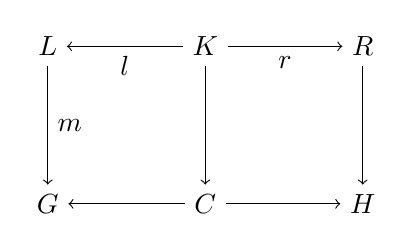
\begin{tikzpicture}
            \node (I) at (0,0) {$K$};
            \node (L)  at (-2,0) {$L$};
            \node (R)  at (2,0) {$R$};
            \node (G)  at (-2,-2) {$G$};
            \node (C)  at (0,-2) {$C$};
            \node (H)  at (2,-2) {$H$};
            \draw [->] (I) to  node [midway,below] {$l$} (L);
            \draw [->] (I) to  node [midway,below] {$r$} (R);
            \draw [->] (L) to node [midway,right] {$m$} (G);
            \draw [->] (I) to  node [midway,right] 
            % {$u$}
            {} (C); 
            \draw [->] (R) to  node [midway,right] 
            {}
            (H);
            \draw [->] (C) to node [midway,above] {} (G);
            \draw [->] (C) to node [midway,above] 
            {} 
            (H);
        \end{tikzpicture}
        }
        \caption{}
        \label{fig:preliminaries:a_rewriting_framework}
\end{figure}
    The \textbf{DPO rewriting relation $\Rightarrow_{\rho,\mathfrak{F}}$ induced by a DPO rewriting rule $\rho$ in $\mathfrak{F}$} is defined as follows:
     $$G \Rightarrow_{\rho,\mathfrak{F}} H \text{if and only if} G \Rightarrow_\rho^\delta H$$
    for some $\delta \in \mathfrak{F}(\rho)$. 
     The \textbf{DPO rewriting relation $\Rightarrow_{\mathcal{R},\mathfrak{F}}$ induced by a set $\mathcal{R}$ of DPO rewriting rules in $\mathfrak{F}$} is given by: 
     $$G \Rightarrow_{\mathcal{R},\mathfrak{F}} H \text{if and only if} G \Rightarrow_{\rho,\mathfrak{F}} H$$ for some $\rho \in \mathcal{R}$. Whenever $\mathfrak{F}$ is clear from the context, we 
    omit $\mathfrak{F}$ and 
    write $\Rightarrow_{\rho}$ and $\Rightarrow_{\mathcal{R}}$.
  \end{definition}
% Let \(\mathfrak{F}\) denote the DPO rewriting framework that associates each rule \( \rho = (L \overset{l}{\leftarrow} K \overset{r}{\rightarrow} R) \) with the collection of all DPO diagrams of the form shown in~\autoref{fig:preliminaries:a_rewriting_framework}.
Throughout this work, we will use the notation \(\mathfrak{M}\) to denote the DPO rewriting framework that associates each rule with the class of all DPO diagrams of the form shown in~\autoref{fig:preliminaries:a_rewriting_framework} with monic match $m$.
